\addtolength{\textheight}{-10pt}

\section{EXPERIMENTS}
\label{sec:experiments}

\subsection{Training}
To train our networks, we used the PyTorch\footnote{\url{https://github.com/pytorch/pytorch}} deep learning framework. The networks were trained using the Adadelta Optimizer \cite{DBLP:journals/corr/abs-1212-5701}.

The loss function used for training and validation was Mean Squared Error  (MSE) Loss. During the training phase, the loss was calculated across all values outputted by the network, i.e., across all ten time steps following the formula
\begin{equation} \label{eq:1}
MSE_{train} = \dfrac{1}{2n}\sum_{t=1}^{n}(s'_t -  s_t)^2 +(m'_t - m_t)^2 
\end{equation}
where $n=10$ is the number of time steps in our case, $s_t$  and $m_t$ are the steering and motor values respectively outputted by the network at a given time step, and $s'_t$ and $p'_t$ are the expert steering and motor values at a given timestep.

During validation, a similar MSE loss metric was used except the loss was calculated only for the two final motor and steering output as given by
\begin{equation} \label{eq:2}
MSE_{validation} = \dfrac{1}{2} (s'_n -  s_n)^2 +(m'_n - m_n)^2
\end{equation}
Only the final timestep was used in measuring the validation accuracy of the networks as this is the only value which is used for evaluation on the model vehicles, and thus the only value which affects the driving performance of the model car. We chose to use the MSE loss function, as small deviations from expert driving were considered normal while larger deviations are reflective of a problem in the network's control and thus have a greater effect on the calculated error. The quadratic error curve of MSE loss allows for such results and closely mimics results from the percentage autonomy metric introduced later in the paper in which small deviations have an inconsequential effect on performance.

The same set of training data were used for each of the networks, as well as the same unseen validation set. All experiments were replicated eight times with randomly initialized networks and shuffled datasets. The results here depict the mean across these trials, with error bars representing 95\% confidence intervals.

Our dataset contains approximately 1.93 million usable data moments for training and validation on the networks. 10\% of the collected data were kept for use in an unseen validation dataset for the evaluation of the networks. All data were equally distributed for each modality in both the training and validation sets. 

\begin{figure}[t]
\centering
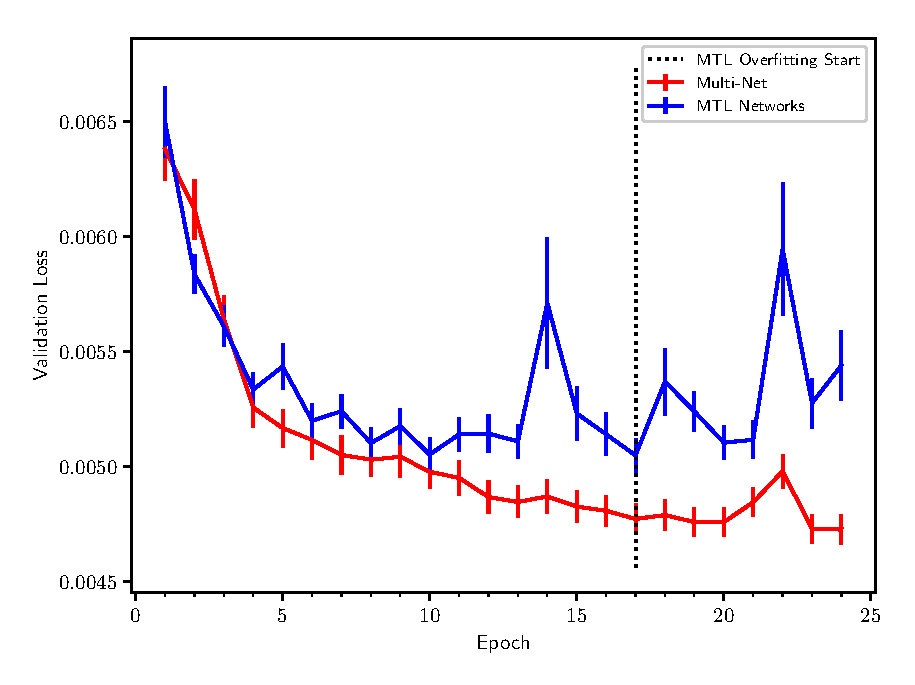
\includegraphics[width=\linewidth]{paper/content/images/mtl}
\caption{Multi-Modal Validation of MultiNet and MTL Networks with 95\% Confidence Intervals}
\label{fig:lve}
\end{figure}

\subsection{Multi-Modal Comparison}
In our initial experiment a MultiNet Z2Color network trained in a multi-modal dataset of direct, follow, and furtive was compared to three MTL Z2Color networks trained on direct, follow, and furtive modes separately. The networks were than evaluated using the validation loss measurement described in \Cref{eq:2}. The results are summarized in \Cref{fig:lve} where the losses of the three MTL networks are averaged across the modes for direct comparison to the MultiNet models.

Initially, from epochs 1 to 4, the MultiNets have similar but slightly poorer performance compared to the MTL networks. This is due to the wide variety of data the MultiNets receive requiring greater generalization initially, while the MTL networks can immediately specialize to specific modes.

From epochs 4 to 10, the MultiNets begin to surpass the MTL networks while remaining close in performance. During this period we hypothesize that the MTL networks begin to differentiate between individual driving modalities by using the provided modal information data.

From epochs 10 to 17, the MultiNets drastically outperform the MTL networks, which flatten off in their loss curve here. The MTL loss curve begins to move erratically by getting caught in various local minima. However it doesn't yet begin overfitting, which we characterize as consistently having a loss value above the absolute minimum. The MultiNets steadily improve through the use of the additional modal data. From epochs 17 to 24, the MTL networks begin to overfit dramatically, while the MultiNets continue to decline in loss despite a small bump at epochs 21 and 22. This suggests MTL networks are more susceptible to overfitting and local minima than their MultiNet counterpart. This is likely due to the variety of data the MultiNet networks are exposed to allowing for greater generalization across modes, while maintaining individual behavioral characteristics in specific modalities.

\begin{figure}[t]
\centering
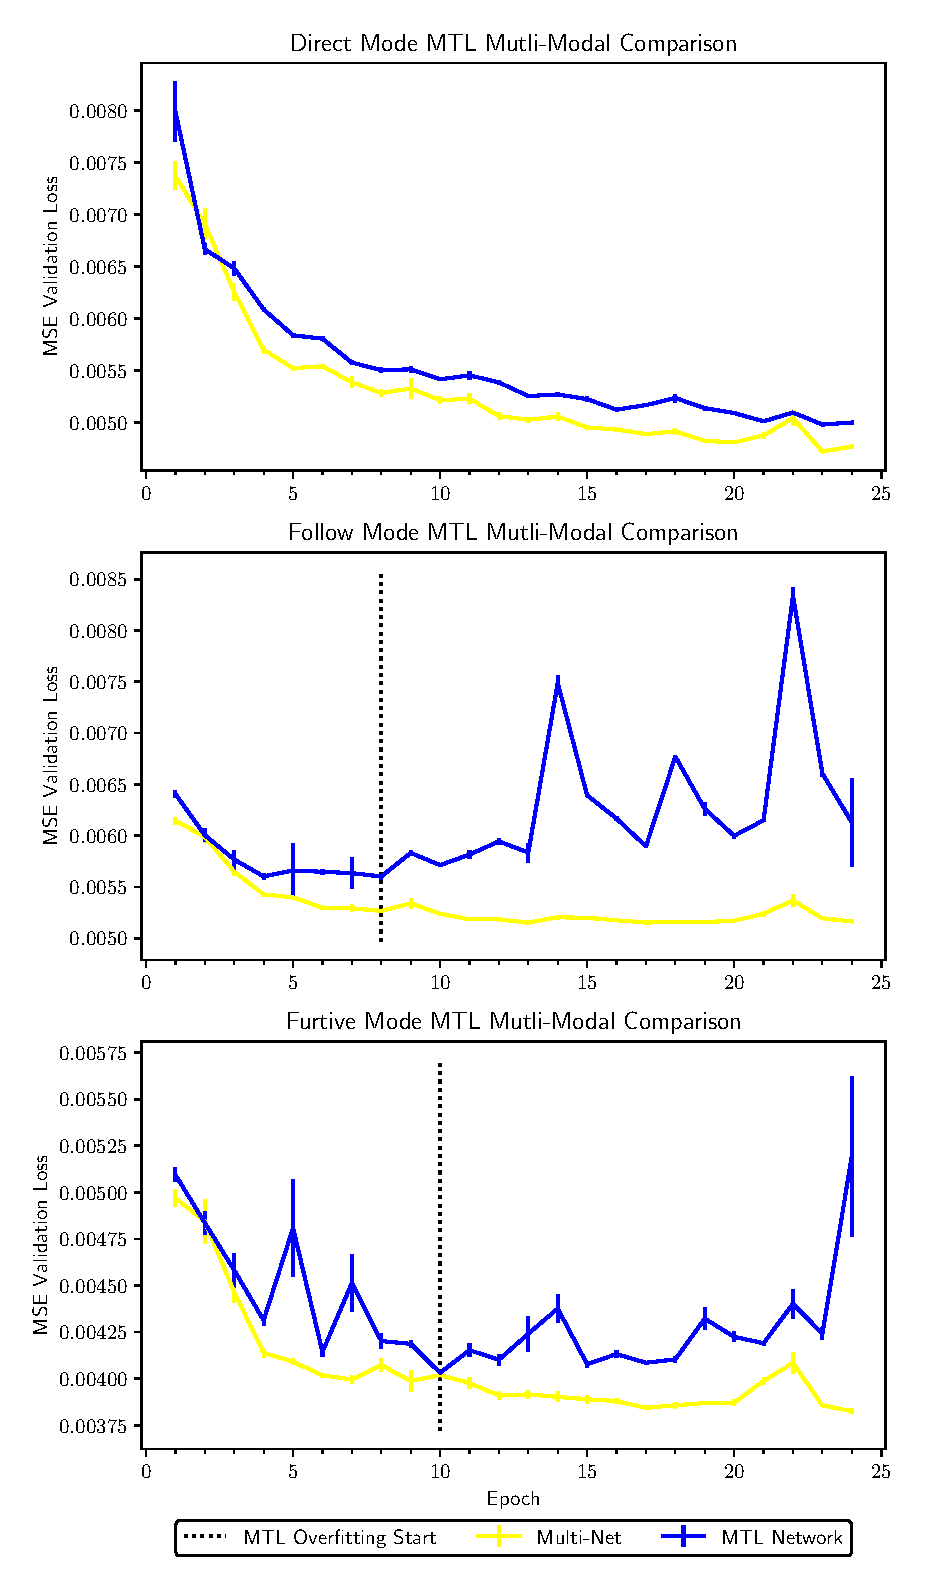
\includegraphics[width=\linewidth]{paper/content/images/individual_new}
\caption{Furtive Mode Validation of MultiNet and MTL Networks with 95\% Confidence Intervals}

\label{fig:furtivegraph}
\end{figure}


\subsection{Performance in Individual Modes}

To further investigate the network's performance in individual behavioral modes, further experiments were done to compare the MultiNet models to a single MTL network in individual modes. These experiments were conducted to evaluate how the MultiNet displays behaviors distinct to the individual driving modes. In the experiments depicted in \Cref{fig:furtivegraph}, the MultiNet models were trained on Direct, Folow, and Furtive data in each experiment while the MTL networks were trained only on the data for that experiment, e.g., for the furtive graph the MTL network was trained and validated on furtive data. Validation was done only on the data for the appropriate mode of each network, e.g., both the MTL and MultiNet models were evaluated only in furtive mode for the furtive graph.

In the first mode, direct mode, it is clear that both networks have similar performance levels. In the second epoch, the MTL networks outperformed the multi net networks, this is likely due to initial confusion between the behavioral modalities in the MultiNet networks. After this point we hypothesize the MultiNet models learnt the modal distinctions and thus continued to have lower loss measurements than their MTL counterparts until the end of training. Both networks seemed to learn the direct mode task quickly and had no large fluctuations in loss or overfitting as compared to the graphs for each of the other modes. This suggests direct mode is the simplest task as it doesn't involve any special behavioral activity and simply involves avoiding obstacles in the vehicle's path. 

In follow mode, the initial performance in the first four epochs is the same as what was observed for direct mode. It is clear that the multi-modal models seemed to require approximately two epochs of training to begin to distinguish between different modes and develop distinct behaviors. Starting from the fifth epoch, the MTL networks began to oscillate rapidly in the recorded validation loss. This suggests that the MTL networks found their minima already and are thus oscillating in this region. After the tenth epoch, the MTL models reached their absolute minimum validation loss.

Initially, from epochs 1 to 4 the MultiNets have similar performance to the furtive networks. From epochs 4 to 10, the MultiNets fall steadily in loss, while the MTL networks oscillate erratically in local minima. From epochs 10 to 24, the MTL networks overfit while the MultiNets continue learning. This demonstrates that for any given mode, a MultiNet network can outperform an MTL network trained for the specific mode.

%This mirrors the results from \Cref{fig:lve}, and confirms the MultiNets resistance to overfitting and local minima as well as their general improved performance.

\subsection{Evaluation on Model Cars}

To test the proficiency of the cars in real world driving situations, we measure the percentage autonomy metric \cite{bojarski2016end} measured as
\begin{equation}
    autonomy = (1 - \dfrac{correction\ time}{elapsed\ time}) \cdot 100
   \label{eq:autonomy}
\end{equation}

MTL and MultiNets were evaluated on a winding 200 m loop of sidewalk (\Cref{fig:evalpath}) with sufficient obstacles within a one hour interval. Follow mode was excluded as driving of the leader car could affect performance of the following car. The networks for on the road evaluation were chosen at the point of absolute minimum average validation error across the trials, i.e., we chose the epoch and trial which minimized the average validation error for both the MultiNet and MTL networks. This minimum occured at epoch 23 on a specific trial, before either network began to overfit. 

The results are summarized as follows: The MultiNet in direct, and furtive mode scored 92.68\% and 88.23\% autonomy respectively. The MTL networks scored 84.27\% and 87.55\% in direct and furtive modes. Comparatively, in direct mode the MultiNet was 8.31 \% more autonomous than the network trained only on direct mode data. In furtive mode the MultiNet was 0.68 \% more autonomous than the MTL net, matching the results from validation on furtive mode and across modes (\Cref{fig:furtivegraph,fig:lve}).
